\documentclass{article}

\usepackage[english]{babel}
\usepackage[utf8]{inputenc}
\usepackage{amsmath,amssymb}
\usepackage{parskip}
\usepackage{graphicx}
\usepackage{listings}
\usepackage{float}
\usepackage{subfig}

% Margins
\usepackage[top=2.5cm, left=3cm, right=3cm, bottom=4.0cm]{geometry}
% Colour table cells
\usepackage[table]{xcolor}

% Get larger line spacing in table
\newcommand{\tablespace}{\\[1.25mm]}
\newcommand\Tstrut{\rule{0pt}{2.6ex}}         % = `top' strut
\newcommand\tstrut{\rule{0pt}{2.0ex}}         % = `top' strut
\newcommand\Bstrut{\rule[-0.9ex]{0pt}{0pt}}   % = `bottom' strut

%%%%%%%%%%%%%%%%%
%     Title     %
%%%%%%%%%%%%%%%%%
\title{CSCI946 Assignment}
\author{Yao Xiao \\ SID 2019180015}
\date{\today}

\begin{document}
\maketitle

%%%%%%%%%%%%%%%%%
%   Problem 1   %
%%%%%%%%%%%%%%%%%
\section{Problem 1}
\begin{lstlisting}
sales <- read.csv("yearly_sales.csv")

head(sales)
summary(sales)

plot(sales$num_of_orders, sales$sales_total, main="Number of Orders vs. Sales")

results <- lm(sales$sales_total ~ sales$num_of_orders)
results
summary(results)
hist(results$residuals, breaks = 800)
\end{lstlisting}

\subsection{Output}
\begin{figure}[H]
    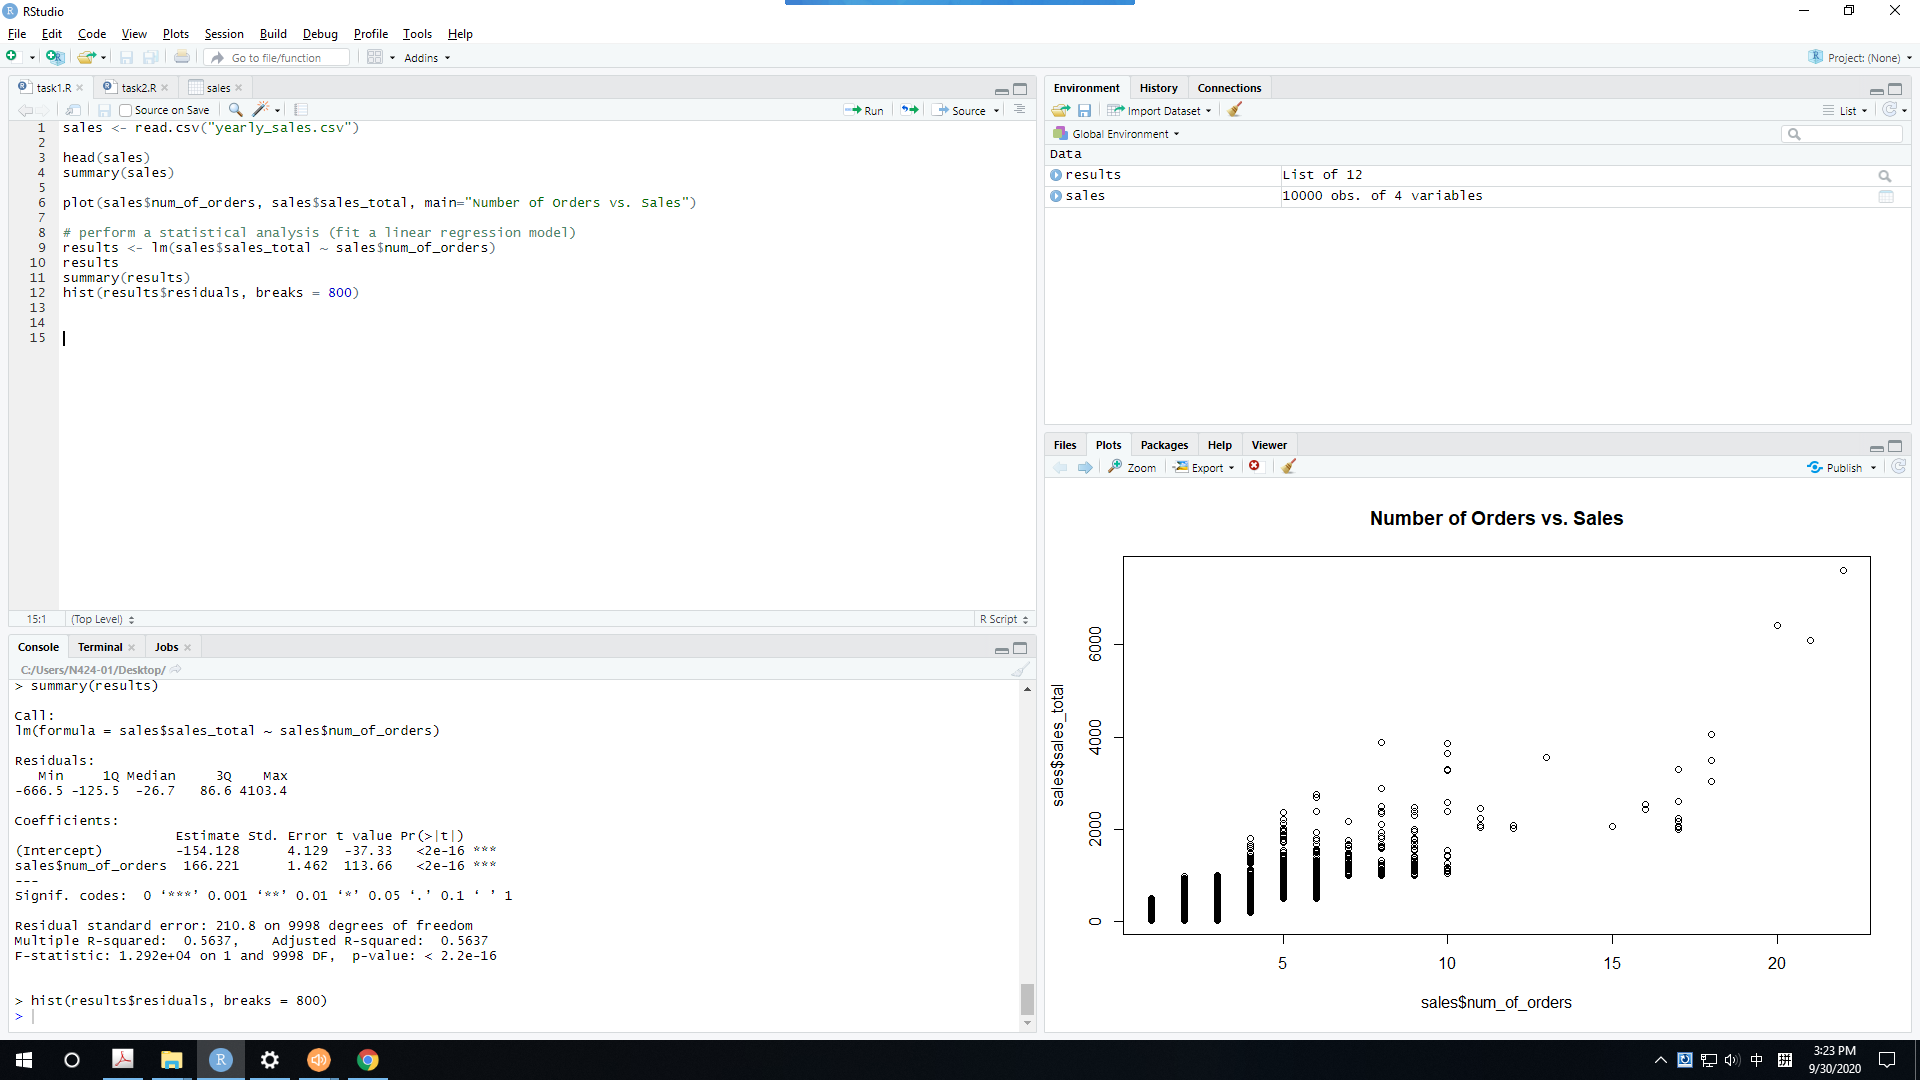
\includegraphics[width=1\textwidth]{Fig1}
\end{figure}

\begin{figure}[H]
    \centering
    \subfloat{
    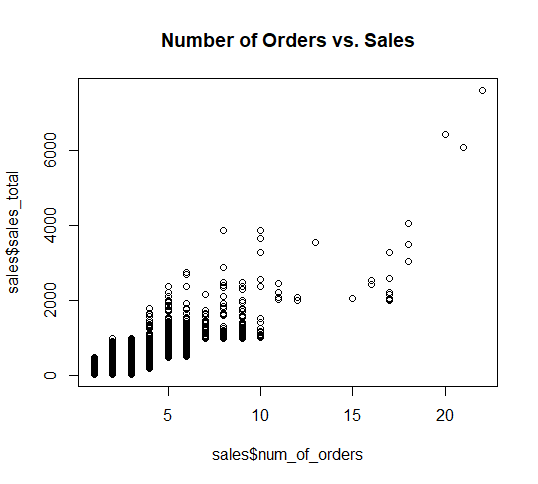
\includegraphics[width=0.5\textwidth]{Rplot.png}
    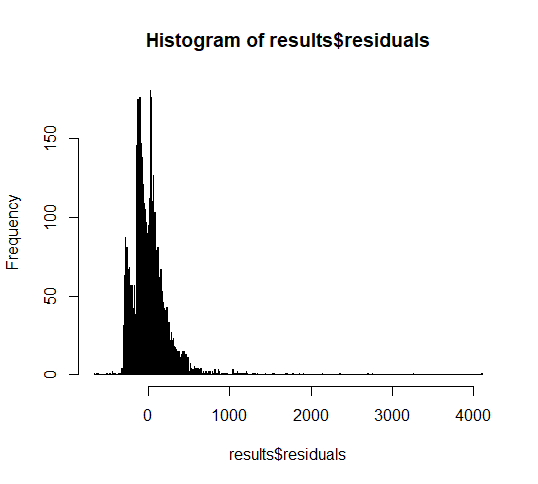
\includegraphics[width=0.5\textwidth]{Rplot01.png}}
\end{figure}



\section{Problem 2}
\begin{lstlisting}
sales <- read.csv("yearly_sales.csv")

sales$per_order <- sales$sales_total/sales$num_of_orders

write.table(sales, "sales_modified.txt", sep="\t", row.names = FALSE)

jpeg(file="sales_hist.jpeg")

hist(sales$num_of_orders)

dev.off()

getwd()

list.files()

View(sales)

ls()

rm(sales)

rm(list=ls())

\end{lstlisting}

\subsection{Output}

\begin{figure}[H]
    \centering
    \subfloat{
        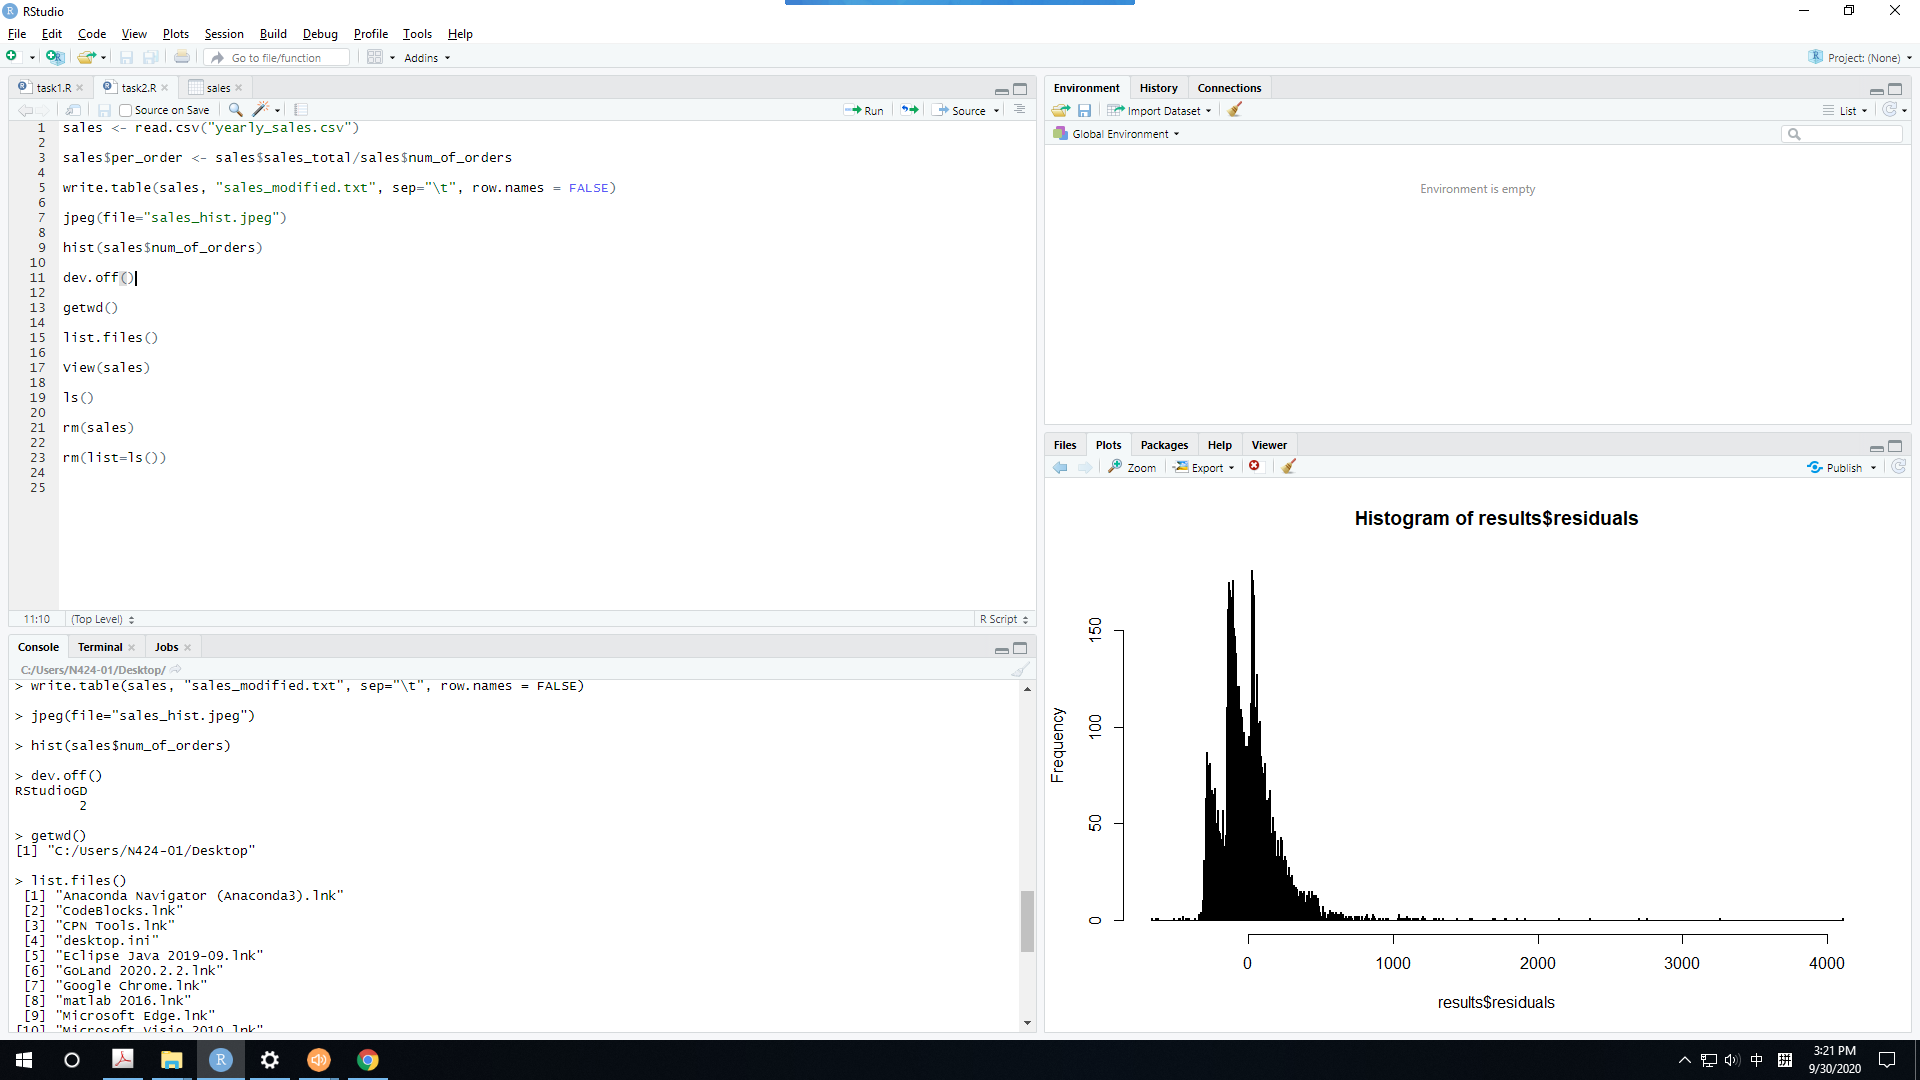
\includegraphics[width=1\textwidth]{Fig2}}
    \newline
    \subfloat{
        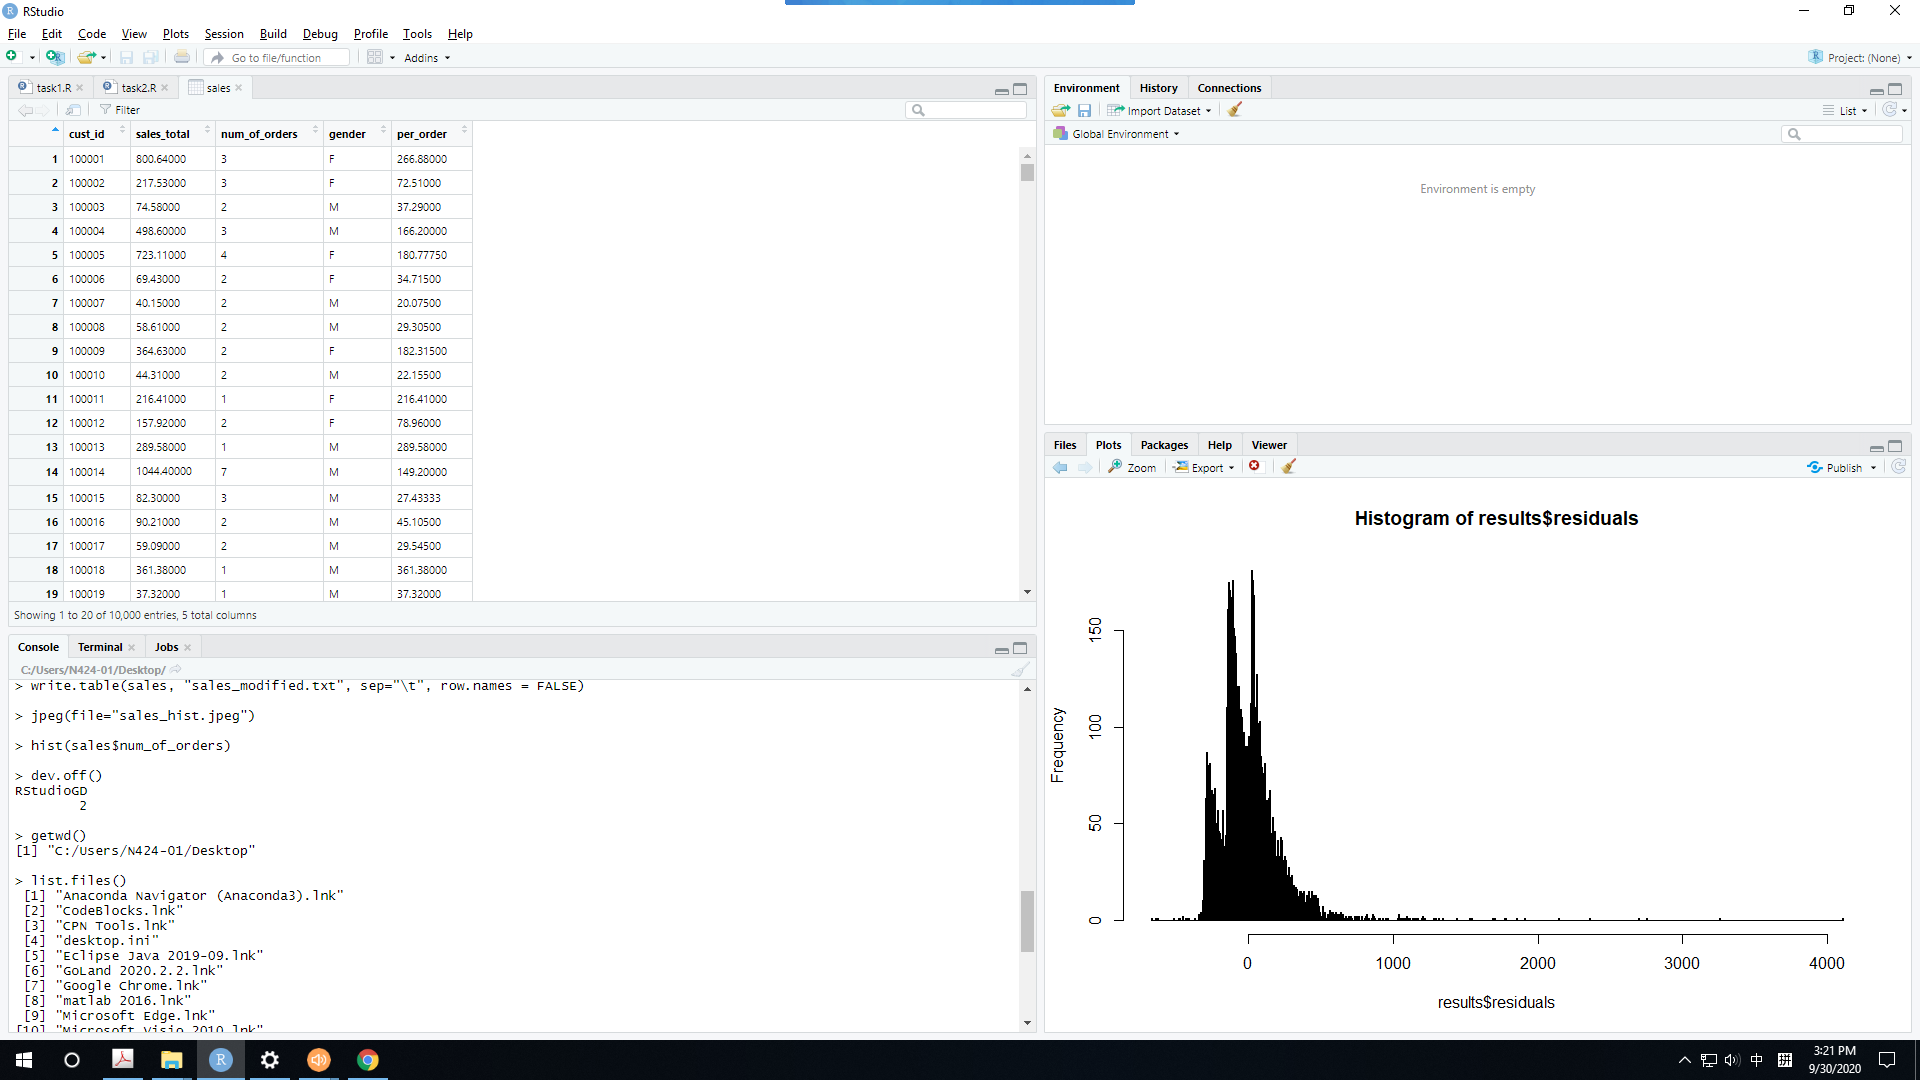
\includegraphics[width=1\textwidth]{Fig3}}
\end{figure}

\begin{figure}[H]
    \centering
    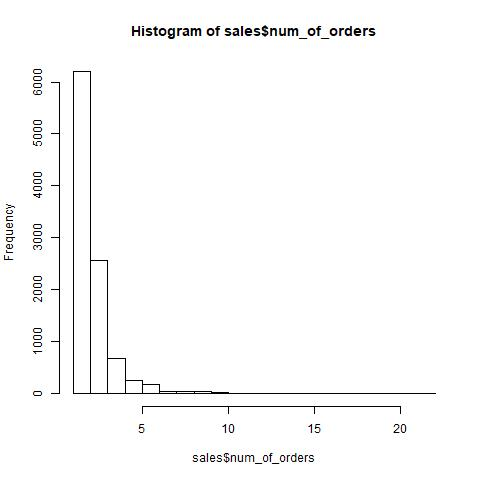
\includegraphics[width=1\textwidth]{sales_hist.jpeg}
\end{figure}



\end{document}